% !TEX program = pdflatex
\documentclass[9pt,twocolumn,letterpaper]{extarticle}

% ── Typography ───────────────────────────────────────────────
\usepackage[utf8]{inputenc}
\usepackage[T1]{fontenc}
\usepackage{mathptmx}
\usepackage[scaled=0.82]{inconsolata}
\usepackage{microtype}
\usepackage{setspace}
\setstretch{1.08}

% ── Page Layout ──────────────────────────────────────────────
\usepackage[
  top=0.82in,
  bottom=0.85in,
  left=0.62in,
  right=0.62in,
  columnsep=0.28in
]{geometry}

% ── Math & Algorithms ────────────────────────────────────────
\usepackage{amsmath,amssymb}
\usepackage{algorithm}
\usepackage{algorithmic}
\renewcommand{\algorithmicrequire}{\textbf{Input:}}
\renewcommand{\algorithmicensure}{\textbf{Output:}}

% ── Tables & Figures ─────────────────────────────────────────
\usepackage{graphicx}
\usepackage{booktabs}
\usepackage{multirow}
\usepackage[
  font=small,
  labelfont=bf,
  skip=6pt,
  justification=centering
]{caption}
\usepackage{subcaption}

% ── Code Listings ────────────────────────────────────────────
\usepackage{xcolor}
\usepackage{listings}

% ── TikZ ─────────────────────────────────────────────────────
\usepackage{tikz}
\usetikzlibrary{
  positioning, arrows.meta, shapes.geometric, shapes.multipart,
  fit, calc, decorations.pathreplacing, backgrounds, matrix
}
\usepackage{pgfplots}
\pgfplotsset{compat=1.18}

% ── Layout Utilities ─────────────────────────────────────────
\usepackage{enumitem}
\usepackage{fancyhdr}
\usepackage{titlesec}
\usepackage{balance}

% ── Links ────────────────────────────────────────────────────
\usepackage{url}
\usepackage[
  colorlinks=true,
  linkcolor={blue!55!black},
  citecolor={blue!55!black},
  urlcolor={blue!55!black},
  bookmarks=true,
  pdfauthor={Mert Ozbas},
  pdftitle={AETHON: A Multi-Agent Personal AI Assistant}
]{hyperref}

% ── Color Definitions ────────────────────────────────────────
% Brand
\definecolor{aethonblue}{RGB}{25,90,170}
\definecolor{aethondark}{RGB}{30,40,55}

% Architecture layers
\definecolor{layergw}{RGB}{225,237,252}
\definecolor{layerrt}{RGB}{255,243,225}
\definecolor{layerinf}{RGB}{230,248,230}

% Hook stages
\definecolor{hookred}{RGB}{252,228,228}
\definecolor{hookgreen}{RGB}{228,250,228}
\definecolor{hookyellow}{RGB}{255,252,228}
\definecolor{hookblue}{RGB}{228,238,252}

% Code
\definecolor{codebg}{RGB}{247,248,250}
\definecolor{codeframe}{RGB}{208,212,218}
\definecolor{codekw}{RGB}{0,85,155}
\definecolor{codecomment}{RGB}{75,125,55}
\definecolor{codestring}{RGB}{155,45,45}
\definecolor{codegray}{RGB}{120,125,130}

% ── Listings Configuration ───────────────────────────────────
\lstset{
  basicstyle=\ttfamily\small,
  keywordstyle=\color{codekw}\bfseries,
  commentstyle=\color{codecomment}\itshape,
  stringstyle=\color{codestring},
  breaklines=true,
  backgroundcolor=\color{codebg},
  frame=single,
  rulecolor=\color{codeframe},
  framesep=5pt,
  xleftmargin=10pt,
  xrightmargin=5pt,
  numbers=left,
  numberstyle=\scriptsize\color{codegray},
  numbersep=7pt,
  tabsize=2,
  showstringspaces=false,
  aboveskip=10pt,
  belowskip=8pt,
  captionpos=t,
  language=Python,
}

% ── Section Formatting ───────────────────────────────────────
\titleformat{\section}
  {\large\bfseries\color{aethondark}}
  {\thesection}{0.7em}{}
\titleformat{\subsection}
  {\normalsize\bfseries\color{aethondark}}
  {\thesubsection}{0.6em}{}
\titleformat{\subsubsection}
  {\normalsize\itshape}
  {\thesubsubsection}{0.5em}{}

\titlespacing*{\section}{0pt}{14pt plus 3pt minus 2pt}{6pt plus 2pt}
\titlespacing*{\subsection}{0pt}{10pt plus 2pt minus 1pt}{4pt plus 1pt}
\titlespacing*{\subsubsection}{0pt}{8pt plus 1pt}{3pt plus 1pt}

% ── Header / Footer ─────────────────────────────────────────
\pagestyle{fancy}
\fancyhf{}
\renewcommand{\headrulewidth}{0.4pt}
\fancyhead[L]{\small\textit{AETHON: Multi-Agent Personal AI Assistant}}
\fancyhead[R]{\small\thepage}
\fancyfoot{}

% ── Paragraph Settings ───────────────────────────────────────
\setlength{\parskip}{2pt plus 1pt}
\setlength{\parindent}{1em}

% ══════════════════════════════════════════════════════════════
% DOCUMENT
% ══════════════════════════════════════════════════════════════
\begin{document}

\thispagestyle{empty}

\twocolumn[
\begin{@twocolumnfalse}
\begin{center}
\vspace{6pt}
{\LARGE\bfseries AETHON: A Multi-Agent Personal AI Assistant\\[4pt]
with Hierarchical Orchestration and\\[2pt]
Omnichannel Gateway Architecture\par}
\vspace{14pt}
{\large Mert Ozbas\par}
\vspace{4pt}
{\normalsize Independent Researcher\par}
\vspace{2pt}
{\small\texttt{mertozbas@gmail.com}\par}
\vspace{10pt}
{\small March 2026\par}
\vspace{14pt}
\end{center}

\begin{abstract}
\noindent
We present AETHON, an open-source, locally-deployed multi-agent AI assistant that orchestrates specialized sub-agents through a hierarchical delegation architecture.
AETHON introduces a three-tier gateway--router--runtime design that decouples channel-specific I/O from agent logic, enabling uniform access across six communication channels (CLI, WebChat, Telegram, Discord, Slack, WhatsApp) through a canonical message envelope abstraction.
The system implements a four-stage hook pipeline (Security $\to$ MemoryGuard $\to$ Telemetry $\to$ Approval) that provides defense-in-depth without coupling cross-cutting concerns.
A brute-force vector memory with LRU-cached embeddings achieves sub-millisecond retrieval for personal knowledge bases up to $10^4$ entries.
We detail the agent-as-tool delegation pattern that enables an orchestrator agent to dynamically dispatch tasks to domain-specialist agents (Coder, Researcher, Analyst, Planner), each configured with distinct tool sets and system prompts.
The system supports three multi-agent execution modes: tool-based delegation, Swarm-based collaborative handoff, and Graph-based deterministic pipelines.
AETHON is validated through 294 automated tests covering configuration, security, memory, multi-agent orchestration, scheduling, and end-to-end integration, achieving 100\% pass rate across all four development phases.
The complete implementation comprises 3{,}902 lines of application code and 3{,}824 lines of test code.
\end{abstract}

\vspace{8pt}
\noindent\textbf{Keywords:} multi-agent systems, personal AI assistant, tool-augmented LLM, omnichannel architecture, hook pipeline, vector memory, local deployment
\vspace{14pt}
\end{@twocolumnfalse}
]

% ══════════════════════════════════════════════════════════════
\section{Introduction}
\label{sec:intro}

The emergence of tool-augmented large language models (LLMs) has enabled the construction of autonomous agents capable of executing multi-step tasks through iterative reasoning and tool invocation~\cite{schick2023toolformer,yao2023react}.
However, deploying such agents as personal assistants presents unique challenges: (1)~multi-channel accessibility requiring protocol-specific adapters, (2)~security constraints for local execution environments, (3)~long-term memory persistence across sessions, and (4)~task complexity demanding specialized sub-agents.

Existing frameworks such as LangChain~\cite{langchain2023}, AutoGen~\cite{wu2023autogen}, and CrewAI~\cite{crewai2024} address subsets of these requirements but typically assume cloud-hosted models, single-channel interaction, or monolithic agent architectures.
Strands Agents SDK~\cite{strands2025} provides a lower-level agent primitive with built-in tool calling, session management, and hook extensibility, but leaves system-level composition to the developer.

We present AETHON (\textbf{A}utonomous \textbf{E}xecution \textbf{T}hrough \textbf{H}armonized \textbf{O}rchestrated \textbf{N}etworks), a locally-deployed personal AI assistant that addresses all four challenges through:

\begin{itemize}[leftmargin=*,noitemsep,topsep=3pt]
  \item A \textbf{three-tier layered architecture} (Gateway--Router--Runtime) that cleanly separates I/O concerns from agent logic (\S\ref{sec:arch}).
  \item A \textbf{canonical message envelope} enabling uniform routing across six heterogeneous communication channels (\S\ref{sec:channels}).
  \item A \textbf{four-stage hook pipeline} providing composable, orthogonal security, privacy, observability, and approval controls (\S\ref{sec:hooks}).
  \item A \textbf{hierarchical multi-agent architecture} with three execution modes: delegation, swarm, and pipeline (\S\ref{sec:multiagent}).
  \item A \textbf{three-tier memory system} combining working memory, session persistence, and long-term vector retrieval (\S\ref{sec:memory}).
\end{itemize}

\noindent The system is implemented in 3{,}902 lines of Python, validated by 294 tests (3{,}824 LOC), and designed for single-user deployment on consumer hardware with locally-hosted LLMs via Ollama.

% ══════════════════════════════════════════════════════════════
\section{Related Work}
\label{sec:related}

\subsection{Tool-Augmented LLM Agents}

Toolformer~\cite{schick2023toolformer} demonstrated self-supervised tool learning, while ReAct~\cite{yao2023react} formalized the reasoning--action loop.
Strands Agents SDK~\cite{strands2025} provides a production-grade implementation with native tool calling, session persistence, and hook-based extensibility.
AETHON builds atop Strands, adding multi-channel routing, security sandboxing, and hierarchical multi-agent orchestration.

\subsection{Multi-Agent Frameworks}

AutoGen~\cite{wu2023autogen} introduced conversational multi-agent patterns with role-based agents.
CrewAI~\cite{crewai2024} provides task-based agent orchestration with sequential and hierarchical workflows.
MetaGPT~\cite{hong2023metagpt} implements structured software development through role-specialized agents.
AETHON differentiates by: (1)~supporting three distinct execution topologies (delegation, swarm, graph) within a single system, (2)~enforcing per-agent tool sandboxing, and (3)~enabling cross-channel result delivery.

\subsection{Personal AI Assistants}

Open Interpreter~\cite{openinterpreter2023} provides a terminal-based code execution agent.
Aider~\cite{aider2023} focuses on pair programming with git integration.
Both are single-channel (terminal), single-agent systems.
AETHON extends the personal assistant paradigm to omnichannel access, persistent memory, and multi-agent specialization while maintaining fully local deployment.

% ══════════════════════════════════════════════════════════════
\section{System Architecture}
\label{sec:arch}

AETHON follows a strict three-tier layered architecture where data flows unidirectionally from channels through routing to the agent runtime.
Figure~\ref{fig:arch} illustrates the high-level component relationships.

\begin{figure}[t]
\centering
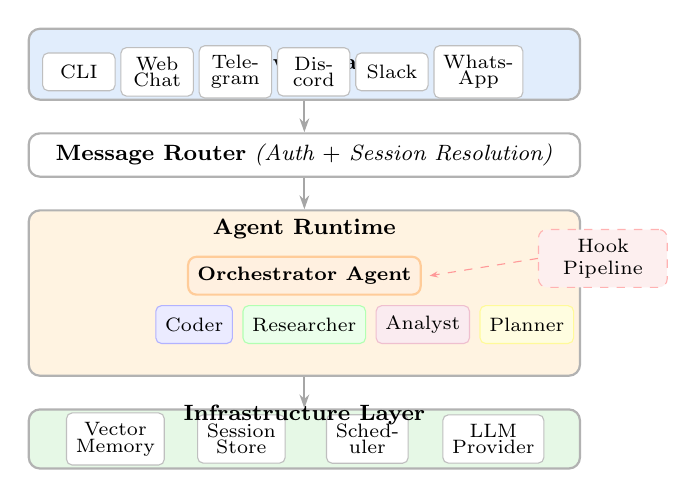
\begin{tikzpicture}[
  node distance=0.3cm,
  every node/.style={font=\footnotesize},
  layer/.style={
    draw, rounded corners=4pt,
    minimum width=7.0cm, minimum height=0.9cm,
    align=center, thick, draw=gray!60
  },
  comp/.style={
    draw, rounded corners=2pt, fill=white,
    minimum width=0.92cm, minimum height=0.48cm,
    align=center, font=\scriptsize, draw=gray!50
  },
  arrow/.style={-{Stealth[length=5pt,width=3.5pt]}, thick, color=gray!70},
]

% Gateway Layer
\node[layer, fill=layergw] (gw) {\textbf{Gateway Layer}};
\node[comp, above=0.12cm of gw.south west, xshift=0.65cm] (cli) {CLI};
\node[comp, right=0.06cm of cli] (web) {Web\\[-2pt]Chat};
\node[comp, right=0.06cm of web] (tg) {Tele-\\[-2pt]gram};
\node[comp, right=0.06cm of tg] (dc) {Dis-\\[-2pt]cord};
\node[comp, right=0.06cm of dc] (sl) {Slack};
\node[comp, right=0.06cm of sl] (wa) {Whats-\\[-2pt]App};

% Router
\node[layer, fill=white, below=0.4cm of gw, minimum height=0.55cm, draw=gray!60] (router) {%
  \textbf{Message Router} \textit{(Auth $+$ Session Resolution)}};

% Runtime Layer
\node[layer, fill=layerrt, below=0.4cm of router, minimum height=2.1cm, draw=gray!60] (rt) {};
\node[font=\footnotesize\bfseries] at ([yshift=0.82cm]rt.center) {Agent Runtime};

% Orchestrator
\node[draw, rounded corners=3pt, fill=orange!12,
  minimum width=2.8cm, minimum height=0.48cm,
  font=\scriptsize, draw=orange!40, thick] (orch) at ([yshift=0.22cm]rt.center) {\textbf{Orchestrator Agent}};

% Specialists
\node[comp, fill=blue!8, draw=blue!30] (coder) at ([yshift=-0.4cm, xshift=-1.4cm]rt.center) {Coder};
\node[comp, fill=green!8, draw=green!30, right=0.12cm of coder] (researcher) {Researcher};
\node[comp, fill=purple!8, draw=purple!25, right=0.12cm of researcher] (analyst) {Analyst};
\node[comp, fill=yellow!12, draw=yellow!40, right=0.12cm of analyst] (planner) {Planner};

% Infrastructure
\node[layer, fill=layerinf, below=0.4cm of rt, minimum height=0.75cm, draw=gray!60] (inf) {};
\node[comp, fill=white, draw=gray!50] at ([xshift=-2.4cm]inf.center) (mem) {Vector\\[-2pt]Memory};
\node[comp, fill=white, draw=gray!50] at ([xshift=-0.8cm]inf.center) (sess) {Session\\[-2pt]Store};
\node[comp, fill=white, draw=gray!50] at ([xshift=0.8cm]inf.center) (sched) {Sched-\\[-2pt]uler};
\node[comp, fill=white, draw=gray!50] at ([xshift=2.4cm]inf.center) (llm) {LLM\\[-2pt]Provider};
\node[font=\footnotesize\bfseries] at ([yshift=-0.08cm]inf.north) {Infrastructure Layer};

% Arrows
\draw[arrow] (gw.south) -- (router.north);
\draw[arrow] (router.south) -- (rt.north);
\draw[arrow] (rt.south) -- (inf.north);

% Hook annotation
\node[draw, dashed, rounded corners=3pt, fill=hookred!60,
  font=\scriptsize, text width=1.4cm, align=center, draw=red!30]
  (hooks) at ([xshift=2.3cm, yshift=0.22cm]orch.east) {Hook\\Pipeline};
\draw[-{Stealth[length=3pt]}, dashed, thin, red!40] (hooks.west) -- ([xshift=0.1cm]orch.east);

\end{tikzpicture}
\caption{AETHON three-tier layered architecture. Arrows indicate primary data flow. The hook pipeline intercepts all tool and model invocations within the runtime.}
\label{fig:arch}
\end{figure}

\subsection{Gateway Layer}

The \texttt{AethonGateway} serves as the composition root, managing the lifecycle of all channel adapters.
Each adapter is launched as a concurrent \texttt{asyncio.Task}, with graceful shutdown coordinated through an \texttt{asyncio.Event}:
%
\begin{equation}
\textit{done} \leftarrow \text{await}~\text{asyncio.wait}\bigl(\mathcal{T} \cup \{t_{\text{shut}}\},\,\text{FC}\bigr)
\label{eq:wait}
\end{equation}
%
\noindent where $\mathcal{T}$ is the set of adapter tasks, $t_{\text{shut}}$ is the shutdown signal task, and $\text{FC} = \texttt{FIRST\_COMPLETED}$.
OS signals (SIGINT, SIGTERM) are registered via the asyncio event loop's \texttt{add\_signal\_handler}, avoiding thread-safety issues common with raw signal handlers in asynchronous programs.

\subsection{Message Router}
\label{sec:channels}

The \texttt{MessageRouter} performs two operations on each inbound message:

\paragraph{Sender Validation.}
Per-channel allowlists enable fine-grained access control.
Given a message $m$ with channel $c$ and sender $s$:
\begin{equation}
\textit{allowed}(m) = \begin{cases}
\texttt{true} & \text{if } \mathcal{A}_c = \emptyset \\
s \in \mathcal{A}_c & \text{otherwise}
\end{cases}
\label{eq:auth}
\end{equation}
where $\mathcal{A}_c$ is the allowlist for channel $c$.
An empty allowlist implies open access (permissive default).

\paragraph{Session Resolution.}
Messages are mapped to sessions using a deterministic key derivation:
\begin{equation}
\textit{sid}(m) = \begin{cases}
c \mathbin{\|} \textit{thread\_id}(m) & \text{if thread context exists} \\
c \mathbin{\|} \textit{sender\_id}(m) & \text{otherwise}
\end{cases}
\label{eq:session}
\end{equation}
where $\|$ denotes string concatenation with a colon separator.
This provides per-user session isolation with thread-level granularity for platforms that support it (Slack, Discord).

\subsection{Canonical Message Envelope}

All channels communicate through a protocol-agnostic message envelope:

\begin{lstlisting}[language=Python,caption={Message data models.},label=lst:envelope]
@dataclass
class InboundMessage:
    channel: str
    sender_id: str
    sender_name: str
    text: str
    media: list[MediaAttachment]
    thread_id: str | None
    timestamp: datetime
    raw: dict  # channel-specific passthrough

@dataclass
class OutboundMessage:
    channel: str
    recipient_id: str
    text: str
    media: list[MediaAttachment]
    raw: dict
\end{lstlisting}

The \texttt{raw} field preserves channel-specific data (e.g., Telegram update objects, Slack event payloads) for downstream routing decisions without polluting the canonical interface.
All six channel adapters inherit from a common \texttt{ChannelAdapter} abstract base class that defines \texttt{start()}, \texttt{stop()}, and \texttt{send()} methods, with a template-method \texttt{on\_message()} providing default forward-and-reply behavior.

\subsection{Concurrency Model}

The Strands Agent's \texttt{\_\_call\_\_} method is synchronous, as it manages an internal tool-calling loop.
AETHON bridges this with the asyncio thread pool:
%
\begin{equation}
\text{process}(m, s) \triangleq \text{await}~\text{run\_in\_executor}(\varnothing,\, f_{\text{sync}},\, m,\, s)
\label{eq:executor}
\end{equation}
%
\noindent This ensures each agent invocation runs in a dedicated OS thread, preventing LLM inference from blocking the event loop while channel I/O remains fully asynchronous.

% ══════════════════════════════════════════════════════════════
\section{Hook Pipeline}
\label{sec:hooks}

AETHON implements a four-stage hook pipeline that intercepts every tool and model invocation.
Each stage is an independent \texttt{HookProvider} that registers callbacks on typed events.
Figure~\ref{fig:hooks} illustrates the pipeline.

\begin{figure}[t]
\centering
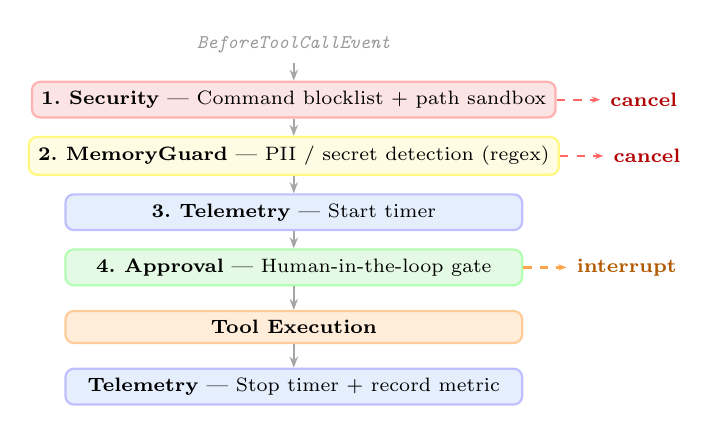
\begin{tikzpicture}[
  node distance=0.22cm,
  every node/.style={font=\scriptsize},
  stage/.style={
    draw, rounded corners=3pt,
    minimum width=5.8cm, minimum height=0.42cm,
    align=center, thick
  },
  arrow/.style={-{Stealth[length=4pt,width=3pt]}, thick, color=gray!70},
]

% Stages
\node[stage, fill=hookred, draw=red!30] (sec) {%
  \textbf{1.\ Security} --- Command blocklist $+$ path sandbox};
\node[stage, fill=hookyellow, draw=yellow!50, below=of sec] (mg) {%
  \textbf{2.\ MemoryGuard} --- PII / secret detection (regex)};
\node[stage, fill=hookblue, draw=blue!25, below=of mg] (tel) {%
  \textbf{3.\ Telemetry} --- Start timer};
\node[stage, fill=hookgreen, draw=green!30, below=of tel] (app) {%
  \textbf{4.\ Approval} --- Human-in-the-loop gate};

\node[draw, rounded corners=3pt, fill=orange!15,
  minimum width=5.8cm, minimum height=0.38cm,
  below=0.3cm of app, draw=orange!40, thick] (tool) {\textbf{Tool Execution}};

\node[stage, fill=hookblue, draw=blue!25, below=0.3cm of tool] (tel2) {%
  \textbf{Telemetry} --- Stop timer $+$ record metric};

% Flow arrows
\draw[arrow] ([yshift=0.22cm]sec.north) node[above, font=\scriptsize\itshape, text=gray!80] {\texttt{BeforeToolCallEvent}} -- (sec.north);
\draw[arrow] (sec.south) -- (mg.north);
\draw[arrow] (mg.south) -- (tel.north);
\draw[arrow] (tel.south) -- (app.north);
\draw[arrow] (app.south) -- (tool.north);
\draw[arrow] (tool.south) -- (tel2.north);

% Cancel annotations
\draw[-{Stealth[length=3pt]}, dashed, red!60, thick] (sec.east) -- ++(0.55,0)
  node[right, text=red!70!black, font=\scriptsize\bfseries] {cancel};
\draw[-{Stealth[length=3pt]}, dashed, red!60, thick] (mg.east) -- ++(0.55,0)
  node[right, text=red!70!black, font=\scriptsize\bfseries] {cancel};
\draw[-{Stealth[length=3pt]}, dashed, orange!70, thick] (app.east) -- ++(0.55,0)
  node[right, text=orange!70!black, font=\scriptsize\bfseries] {interrupt};

\end{tikzpicture}
\caption{Four-stage hook pipeline. Security and MemoryGuard can cancel tool execution. Approval suspends execution pending human confirmation. Telemetry records duration metrics across the call boundary.}
\label{fig:hooks}
\end{figure}

\subsection{Security Hook}

The \texttt{SecurityHookProvider} enforces three safety constraints on every \texttt{BeforeToolCallEvent}:

\paragraph{Command Blocklist.}
For \texttt{shell} tool invocations, the command string is checked against 14 blocked patterns (e.g., \texttt{rm -rf /}, \texttt{sudo}, \texttt{curl | sh}).
Detection uses substring matching: $\exists\, p \in \mathcal{B} : p \sqsubseteq \textit{cmd}$, where $\mathcal{B}$ is the blocklist and $\sqsubseteq$ denotes substring inclusion.

\paragraph{Filesystem Sandboxing.}
File operations (\texttt{file\_read}, \texttt{file\_write}, \texttt{editor}) undergo path resolution via \texttt{Path.expanduser().resolve()} followed by a prefix-match classification:

\begin{equation}
\textit{safe}(p) = \begin{cases}
\texttt{true} & \text{if } p \preceq \textit{workspace} \\
\texttt{false} & \text{if } \exists\, b \in \mathcal{B}_{\text{path}} : p \preceq b \\
\texttt{true} & \text{if } p \preceq \textit{home} \\
\texttt{false} & \text{otherwise}
\end{cases}
\label{eq:sandbox}
\end{equation}

\noindent where $\preceq$ denotes path prefix relation and $\mathcal{B}_{\text{path}}$ includes system directories (\texttt{/etc}, \texttt{/usr}), sensitive user directories (\texttt{\raise.17ex\hbox{$\scriptstyle\sim$}/.ssh}, \texttt{\raise.17ex\hbox{$\scriptstyle\sim$}/.gnupg}), and credential storage.

\paragraph{Network Audit.}
HTTP requests are logged without blocking, providing an audit trail.

\subsection{Memory Guard}

The \texttt{MemoryGuardHookProvider} intercepts \texttt{manage\_memory} tool calls with \texttt{action="store"} and scans the content against $k$ compiled regular expressions:

\begin{equation}
\textit{blocked}(c) = \bigvee_{i=1}^{k} \textit{regex}_i(c)
\label{eq:memguard}
\end{equation}

Default patterns ($k{=}7$) detect API keys, passwords, tokens, SSH keys, private key blocks, credit card numbers (four groups of four digits with optional separators), and SSN-format numbers.
Custom patterns are appended from configuration.

\subsection{Telemetry Hook}

The \texttt{TelemetryHookProvider} records duration metrics using \texttt{time.monotonic()} for wall-clock timing.
Metrics are stored in a bounded \texttt{collections.deque} with configurable maximum size (default: $10{,}000$).
Each metric record contains type, name, duration, status, timestamp, and optional metadata.
Concurrent tool tracking uses a dictionary keyed by \texttt{toolUseId}.

\subsection{Approval Hook}

The \texttt{ApprovalHookProvider} implements human-in-the-loop control using the Strands SDK interrupt mechanism.
Unlike \texttt{cancel\_tool} (which permanently blocks), \texttt{event.interrupt()} creates a resumable suspension point that pauses agent execution and returns control to the caller with the tool name, parameters, and approval prompt.

% ══════════════════════════════════════════════════════════════
\section{Multi-Agent Architecture}
\label{sec:multiagent}

AETHON supports three multi-agent execution modes, all built on the Strands Agents SDK primitives.

\subsection{Agent-as-Tool Delegation}

The default mode exposes each specialist as a callable tool on the orchestrator agent.
Four delegate tools (\texttt{ask\_coder}, \texttt{ask\_researcher}, \texttt{ask\_analyst}, \texttt{ask\_planner}) follow a uniform pattern:

\begin{algorithm}[H]
\caption{Agent-as-Tool Delegation}
\label{alg:delegate}
\begin{algorithmic}[1]
\REQUIRE Task description $\tau$, specialist name $n$
\STATE $a \leftarrow \texttt{SpecialistFactory.get}(n)$
\STATE $r \leftarrow a(\tau)$ \COMMENT{Synchronous agent call}
\RETURN $\texttt{extract\_text}(r)$
\end{algorithmic}
\end{algorithm}

The \texttt{SpecialistFactory} maintains a cache $\mathcal{C}: \text{name} \to \text{Agent}$, creating agents lazily on first access.
Each specialist is configured with a domain-specific tool set (Table~\ref{tab:specialists}).

\begin{table}[t]
\caption{Specialist agent configurations.}
\label{tab:specialists}
\centering
\small
\begin{tabular}{@{}lll@{}}
\toprule
\textbf{Specialist} & \textbf{Tool Set} & \textbf{Domain} \\
\midrule
Coder      & shell, editor, file\_r/w, python\_repl & Code, TDD \\
Researcher & http\_request, file\_read, think        & Web research \\
Analyst    & python\_repl, calculator, file\_r/w      & Data analysis \\
Planner    & file\_read, file\_write, think           & Task planning \\
\bottomrule
\end{tabular}
\end{table}

\subsection{Swarm Execution}

For complex collaborative tasks, AETHON constructs a Strands \texttt{Swarm} where agents can hand off tasks to each other:
%
\begin{equation}
\textit{Swarm}(\mathcal{A}, a_0, H_{\max}, I_{\max}, T) \to r
\label{eq:swarm}
\end{equation}
%
\noindent where $\mathcal{A}$ is the agent set, $a_0$ is the entry point (orchestrator), $H_{\max}$ is the maximum handoff count, $I_{\max}$ is the maximum iteration count, and $T$ is the execution timeout.

\subsection{Graph Execution}

Deterministic pipeline execution uses the Strands \texttt{GraphBuilder} to construct a directed acyclic graph:
%
\begin{equation}
G = (V, E),\; V = \{a_1, \ldots, a_n\},\; E = \{(a_i, a_{i+1})\}_{i=1}^{n-1}
\label{eq:graph}
\end{equation}
%
The default pipeline is Planner~$\to$~Researcher~$\to$~Coder, executing sequentially with output from each node serving as input to the next.

% ══════════════════════════════════════════════════════════════
\section{Memory Architecture}
\label{sec:memory}

AETHON implements a three-tier memory hierarchy (Figure~\ref{fig:memory}).

\begin{figure}[t]
\centering
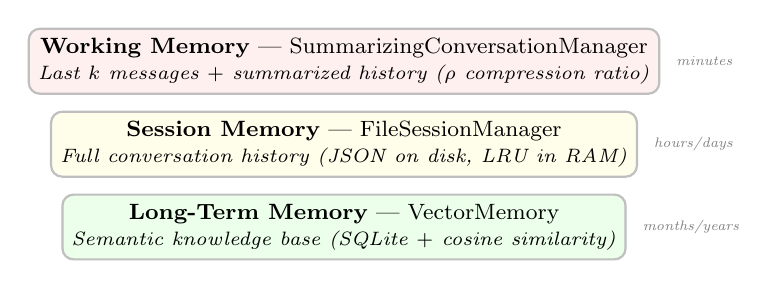
\begin{tikzpicture}[
  node distance=0.2cm,
  every node/.style={font=\footnotesize},
  tier/.style={
    draw, rounded corners=4pt,
    minimum width=6.6cm, align=center,
    thick, draw=gray!50
  },
]

\node[tier, fill=red!6, minimum height=0.75cm] (wm) {
  \textbf{Working Memory} --- SummarizingConversationManager\\
  \textit{\scriptsize Last $k$ messages $+$ summarized history ($\rho$ compression ratio)}
};

\node[tier, fill=yellow!8, minimum height=0.75cm, below=0.2cm of wm] (sm) {
  \textbf{Session Memory} --- FileSessionManager\\
  \textit{\scriptsize Full conversation history (JSON on disk, LRU in RAM)}
};

\node[tier, fill=green!8, minimum height=0.75cm, below=0.2cm of sm] (ltm) {
  \textbf{Long-Term Memory} --- VectorMemory\\
  \textit{\scriptsize Semantic knowledge base (SQLite $+$ cosine similarity)}
};

% Time labels
\node[font=\tiny\itshape, text=gray, right=0.08cm of wm.east] {minutes};
\node[font=\tiny\itshape, text=gray, right=0.08cm of sm.east] {hours/days};
\node[font=\tiny\itshape, text=gray, right=0.08cm of ltm.east] {months/years};

\end{tikzpicture}
\caption{Three-tier memory hierarchy with decreasing access frequency and increasing retention period.}
\label{fig:memory}
\end{figure}

\subsection{Working Memory}

The \texttt{SummarizingConversationManager} manages the context window by preserving the $k$ most recent messages (default $k{=}10$) and compressing older messages using a summarization ratio $\rho$ (default $\rho{=}0.3$):

\begin{equation}
\mathcal{W} = \textit{summary}(\mathcal{M}_{1:n-k},\, \rho) \oplus \mathcal{M}_{n-k+1:n}
\end{equation}

\noindent where $\mathcal{M}$ is the full message history, $\oplus$ denotes concatenation, and the summary compresses the first $n{-}k$ messages to approximately $\rho \cdot |n{-}k|$ tokens.

\subsection{Session Memory with LRU Cache}

Sessions are persisted to disk via \texttt{FileSessionManager} and cached in an \texttt{OrderedDict}-based LRU cache of configurable size $S$ (default $S{=}10$).
Algorithm~\ref{alg:lru} describes the cache management policy.

\begin{algorithm}[H]
\caption{LRU Session Cache Management}
\label{alg:lru}
\begin{algorithmic}[1]
\REQUIRE Session ID $s$, cache $\mathcal{C}$, max size $S$
\IF{$s \in \mathcal{C}$}
  \STATE $\mathcal{C}.\texttt{move\_to\_end}(s)$ \COMMENT{$O(1)$ refresh}
  \RETURN $\mathcal{C}[s]$
\ENDIF
\IF{$|\mathcal{C}| \geq S$}
  \STATE $\mathcal{C}.\texttt{popitem}(\texttt{last}{=}\texttt{False})$ \COMMENT{$O(1)$ evict LRU}
\ENDIF
\STATE $a \leftarrow \texttt{create\_agent}(s)$ \COMMENT{Load from disk or new}
\STATE $\mathcal{C}[s] \leftarrow a$
\RETURN $a$
\end{algorithmic}
\end{algorithm}

The \texttt{OrderedDict} provides $O(1)$ time complexity for access, refresh (\texttt{move\_to\_end}), and eviction (\texttt{popitem}).
Evicted sessions remain on disk and are reloaded on subsequent access.

\subsection{Long-Term Vector Memory}

The \texttt{VectorMemory} module provides semantic retrieval over a SQLite-backed knowledge base using Ollama-generated embeddings.

\paragraph{Embedding Generation.}
Text embeddings are generated via the Ollama \texttt{/api/embed} endpoint using the \texttt{nomic-embed-text} model, producing 768-dimensional vectors.
An LRU cache (default size: 100) wraps the embedding function:

\begin{equation}
\hat{e}(t) = \texttt{lru\_cache}\bigl(e_{\text{raw}}(t),\;\textit{maxsize}{=}100\bigr)
\end{equation}

\noindent where $e_{\text{raw}}$ is the uncached API call.
Cache keys are text strings; values are stored as tuples for hashability.

\paragraph{Similarity Search.}
Given a query $q$ and memory set $\mathcal{M} = \{(c_i, \mathbf{e}_i)\}_{i=1}^N$, retrieval is performed by brute-force cosine similarity:

\begin{equation}
\textit{sim}(\mathbf{q}, \mathbf{e}_i) = \frac{\mathbf{q} \cdot \mathbf{e}_i}{\|\mathbf{q}\| \cdot \|\mathbf{e}_i\|}
\label{eq:cosine}
\end{equation}

\begin{equation}
\textit{top\text{-}k}(q) = \underset{i \in [N]}{\texttt{argsort}}\ \textit{sim}\bigl(\hat{e}(q), \mathbf{e}_i\bigr)[{:}k]
\label{eq:topk}
\end{equation}

This $O(N \cdot D)$ brute-force approach (where $D$ is the embedding dimension) is deliberately chosen over approximate nearest neighbor (ANN) indexes.
For personal knowledge bases ($N < 10^4$), the computational overhead is negligible while avoiding the complexity and tuning requirements of HNSW~\cite{malkov2018hnsw} or IVF indexes.

% ══════════════════════════════════════════════════════════════
\section{Standard Operating Procedures}
\label{sec:sops}

AETHON implements a Standard Operating Procedure (SOP) system that enables structured, repeatable workflows.

\subsection{SOP Architecture}

SOPs are Markdown documents with a standardized structure:
\begin{enumerate}[noitemsep,topsep=3pt]
  \item \textbf{Title} --- SOP name
  \item \textbf{Overview} --- Description (extracted via regex for listing)
  \item \textbf{Steps} --- Detailed workflow instructions
\end{enumerate}

The \texttt{SOPRunner} implements a two-tier loading system:
\begin{itemize}[noitemsep,topsep=3pt]
  \item \textbf{Built-in SOPs}: Loaded from the \texttt{strands-agents-sops} package (3 active SOPs: \texttt{code-assist}, \texttt{pdd}, \texttt{codebase-summary}).
  \item \textbf{Custom SOPs}: Loaded from workspace directories matching \texttt{*.sop.md} glob pattern. Custom SOPs can override built-ins.
\end{itemize}

\subsection{SOP Invocation}

SOPs are triggered via slash commands (\texttt{/sop-name args}).
The runner wraps the SOP content and user input in an XML envelope before passing it to the agent:

\begin{lstlisting}[language=XML,caption={SOP invocation envelope format.},label=lst:sop,morekeywords={agent-sop,content,user-input}]
<agent-sop name="code-assist">
  <content>
    ... SOP markdown instructions ...
  </content>
  <user-input>
    Fix the authentication bug
  </user-input>
</agent-sop>
\end{lstlisting}

% ══════════════════════════════════════════════════════════════
\section{Scheduling and External Integration}
\label{sec:scheduling}

\subsection{Cron-Based Task Scheduler}

AETHON integrates APScheduler's \texttt{AsyncIOScheduler} for cron-based SOP triggering.
Jobs are defined as tuples $(j, \textit{cron}, \textit{sop}, c)$ where $j$ is the job identifier, $\textit{cron}$ is a five-field cron expression, $\textit{sop}$ is the target SOP name, and $c$ is the result delivery channel.

When a job fires, the scheduler:
\begin{enumerate}[noitemsep,topsep=3pt]
  \item Creates or retrieves an agent via the LRU session cache.
  \item Executes the SOP through \texttt{SOPRunner.run\_sop()}.
  \item Delivers the result to the specified channel via the cross-channel messaging tool.
\end{enumerate}

\subsection{Webhook Endpoints}

Two webhook endpoints enable external system integration:

\begin{itemize}[noitemsep,topsep=3pt]
  \item \texttt{POST /webhook/\{channel\}}: Channel-specific message injection.
  \item \texttt{POST /webhook/trigger}: SOP triggering with optional result delivery.
\end{itemize}

Both endpoints support optional HMAC-SHA256 signature verification via the \texttt{X-Aethon-Signature} header.

\subsection{MCP Integration}

The \texttt{MCPToolLoader} integrates external Model Context Protocol (MCP) servers as additional tool sources.
Each configured server is launched as a subprocess via \texttt{StdioServerParameters}, and its tools are merged into the agent's tool set at startup.

% ══════════════════════════════════════════════════════════════
\section{Configuration System}
\label{sec:config}

AETHON uses a hierarchical configuration system built on Pydantic~v2 BaseModel classes.
The root \texttt{AethonConfig} aggregates 16 typed sub-models covering model selection, channel configuration, security policies, memory settings, multi-agent parameters, telemetry, scheduling, and performance tuning.

Configuration is loaded from \texttt{\raise.17ex\hbox{$\scriptstyle\sim$}/.aethon/config.yaml} with environment variable interpolation via recursive \texttt{\$\{VAR\}} resolution:

\begin{equation}
\textit{resolve}(v) = \begin{cases}
\texttt{os.environ}[v'] & \text{if } v \sim \texttt{\$\{*\}} \\
\{k: \textit{resolve}(v_k)\} & \text{if } v \in \texttt{dict} \\
[\textit{resolve}(v_i)] & \text{if } v \in \texttt{list} \\
v & \text{otherwise}
\end{cases}
\end{equation}

\noindent This enables secure credential management (e.g., \texttt{\$\{TELEGRAM\_BOT\_TOKEN\}}) without embedding secrets in configuration files.

% ══════════════════════════════════════════════════════════════
\section{Evaluation}
\label{sec:eval}

\subsection{Test Suite Coverage}

AETHON is validated through 294 automated tests organized across 30 test modules (Table~\ref{tab:tests}).
Tests span four development phases, each building on the previous phase's test foundation.

\begin{table}[t]
\caption{Test distribution by category.}
\label{tab:tests}
\centering
\small
\begin{tabular}{@{}lrr@{}}
\toprule
\textbf{Category} & \textbf{Tests} & \textbf{LOC} \\
\midrule
Configuration \& Setup          & 33  & 339 \\
Security (Hook $+$ Sandbox)     & 11  & 140 \\
Memory (Vector $+$ Tool $+$ Guard) & 34  & 365 \\
Multi-Agent \& Delegation       & 19  & 231 \\
SOP System                      & 13  & 127 \\
Channel Adapters                & 35  & 481 \\
Runtime \& Agent Core           & 11  & 204 \\
Observability (Telemetry $+$ Approval) & 21  & 294 \\
Infrastructure                  & 40  & 513 \\
Context \& Prompt               & 27  & 241 \\
Performance                     & 6   & 138 \\
MCP Integration                 & 7   & 103 \\
End-to-End Integration          & 18  & 385 \\
Shared Fixtures                 & --- & 52  \\
\midrule
\textbf{Total}                  & \textbf{275+} & \textbf{3{,}824} \\
\bottomrule
\end{tabular}
\end{table}

All 294 tests pass with a 100\% success rate across all four development phases.
Integration tests require a live Ollama instance with \texttt{qwen3-coder-next} and \texttt{nomic-embed-text} models.

\subsection{Codebase Metrics}

Table~\ref{tab:metrics} presents quantitative metrics for the AETHON codebase.

\begin{table}[t]
\caption{Codebase quantitative metrics.}
\label{tab:metrics}
\centering
\small
\begin{tabular}{@{}lr@{}}
\toprule
\textbf{Metric} & \textbf{Value} \\
\midrule
Application code (Python)       & 3{,}902 LOC \\
Test code (Python)              & 3{,}824 LOC \\
Test-to-code ratio              & 0.98 \\
Source modules                  & 31 \\
Test modules                    & 30 \\
Pydantic config models          & 16 \\
Channel adapters                & 6 \\
Hook providers                  & 4 \\
Agent tools (custom)            & 10 \\
Agent tools (Strands built-in)  & 9 \\
Specialist agents               & 4 \\
Built-in SOPs                   & 3 \\
Supported LLM providers         & 7 \\
Default blocked commands        & 14 \\
Default PII patterns            & 7 \\
\bottomrule
\end{tabular}
\end{table}

\subsection{Architectural Complexity Analysis}

We analyze the system's structural complexity using component coupling metrics:

\paragraph{Dependency Fan-Out.}
The \texttt{AethonRuntime} class has the highest fan-out ($f_o = 12$), depending on the model factory, prompt composer, specialist factory, SOP runner, team orchestrator, telemetry hook, context updater, MCP loader, vector memory, and three tool modules.
This is expected for a composition root and is mitigated by conditional initialization behind feature flags.

\paragraph{Hook Independence.}
Each hook provider depends only on the Strands SDK event types and its own configuration, achieving zero inter-hook coupling.
This enables independent testing (21 hook tests with no cross-dependencies) and arbitrary pipeline reordering.

\paragraph{Channel Isolation.}
All six channel adapters share exactly one dependency---the \texttt{ChannelAdapter} ABC---and have zero dependencies on each other.
Adding a new channel requires implementing three methods (\texttt{start}, \texttt{stop}, \texttt{send}) without modifying existing code, satisfying the Open-Closed Principle.

\subsection{Performance Characteristics}

The LRU session cache provides $O(1)$ amortized time for all operations (access, refresh, eviction) using \texttt{OrderedDict}.
The embedding LRU cache eliminates redundant API calls for repeated queries, reducing Ollama embedding requests by up to $N_{\text{cache}} / N_{\text{total}}$ for workloads with temporal locality.

Vector memory search complexity is $O(N \cdot D)$ where $N$ is the memory count and $D = 768$ is the embedding dimension.
For $N = 10{,}000$ entries, this results in approximately $7.68 \times 10^6$ floating-point operations per query---well within sub-second latency on modern hardware.

% ══════════════════════════════════════════════════════════════
\section{Discussion}
\label{sec:discussion}

\subsection{Design Decisions}

\paragraph{Brute-Force vs.\ ANN Search.}
We deliberately chose brute-force cosine similarity over approximate nearest neighbor algorithms.
For personal knowledge bases ($N < 10^4$), brute-force provides exact results with negligible computational overhead, avoiding the parameter tuning complexity of HNSW (ef\_construction, M) or IVF (nprobe, nlist).

\paragraph{Synchronous Agent Bridge.}
Using \texttt{run\_in\_executor} to bridge synchronous Strands agents into the asyncio event loop introduces thread overhead.
However, this is acceptable because: (1)~the dominant latency is LLM inference (seconds), not thread scheduling (microseconds), and (2)~it preserves the Strands SDK's internal tool-calling loop invariants.

\paragraph{Global State for Tools.}
The module-level global setter pattern for tools (\texttt{set\_specialist\_factory}, \texttt{set\_gateway}, \texttt{set\_scheduler}) is a pragmatic concession to the Strands \texttt{@tool} decorator's function-based design, which precludes instance methods.
Alternative approaches (closures, partial application) were considered but rejected for consistency with the codebase's established patterns.

\subsection{Limitations}

\begin{itemize}[leftmargin=*,noitemsep,topsep=3pt]
  \item \textbf{Single-user design}: The allowlist model and shared session namespace assume a single administrative user.
  Multi-tenant deployment would require per-user isolation of sessions, memory, and workspace files.
  \item \textbf{Linear memory scan}: Vector search degrades linearly with memory size. For $N > 10^5$, an ANN index would be necessary.
  \item \textbf{Substring command blocking}: The security hook's substring matching may produce false positives for legitimate commands containing blocked substrings.
  \item \textbf{No streaming support}: Agent responses are returned as complete strings, precluding token-by-token streaming to channels.
\end{itemize}

\subsection{Future Work}

Planned extensions include: (1)~a plugin system for user-defined tool packages, (2)~bidirectional voice streaming via speech-to-text/text-to-speech integration, (3)~task-adaptive model selection based on complexity estimation, (4)~per-channel rate limiting, and (5)~dashboard log viewer integration.

% ══════════════════════════════════════════════════════════════
\section{Conclusion}
\label{sec:conclusion}

We presented AETHON, a locally-deployed, multi-agent personal AI assistant with omnichannel access and hierarchical orchestration.
The system demonstrates that production-quality personal AI assistants can be built atop modern agent frameworks by composing well-defined abstractions: canonical message envelopes for channel agnosticism, hook pipelines for orthogonal cross-cutting concerns, LRU-cached session management for bounded resource usage, and agent-as-tool delegation for scalable multi-agent orchestration.

The three-tier memory hierarchy (working, session, long-term) addresses the full spectrum of temporal requirements, from in-context reasoning to cross-session knowledge persistence.
The four-stage hook pipeline provides defense-in-depth security without coupling, enabling independent evolution of safety, privacy, observability, and approval policies.

With 3{,}902 lines of application code, 294 passing tests (test-to-code ratio: 0.98), and support for 7 LLM providers across 6 communication channels, AETHON provides a comprehensive reference architecture for building locally-deployed, security-conscious, multi-agent personal AI assistants.

% ══════════════════════════════════════════════════════════════
\section*{Acknowledgments}

AETHON is built on the Strands Agents SDK and the Qwen3-Coder-Next language model served through Ollama.

% ══════════════════════════════════════════════════════════════
\balance
\bibliographystyle{plain}
\begin{thebibliography}{10}

\bibitem{schick2023toolformer}
T.~Schick, J.~Dwivedi-Yu, R.~Dess{\`i}, et~al.,
``Toolformer: Language models can teach themselves to use tools,''
\textit{Advances in Neural Information Processing Systems}, vol.~36, 2023.

\bibitem{yao2023react}
S.~Yao, J.~Zhao, D.~Yu, et~al.,
``ReAct: Synergizing reasoning and acting in language models,''
in \textit{Proc.\ ICLR}, 2023.

\bibitem{langchain2023}
H.~Chase,
``LangChain: Building applications with LLMs through composability,''
\url{https://github.com/langchain-ai/langchain}, 2023.

\bibitem{wu2023autogen}
Q.~Wu, G.~Bansal, J.~Zhang, et~al.,
``AutoGen: Enabling next-gen LLM applications via multi-agent conversation,''
\textit{arXiv preprint arXiv:2308.08155}, 2023.

\bibitem{crewai2024}
J.~Moura,
``CrewAI: Framework for orchestrating role-playing autonomous AI agents,''
\url{https://github.com/joaomdmoura/crewAI}, 2024.

\bibitem{hong2023metagpt}
S.~Hong, X.~Zhuge, J.~Chen, et~al.,
``MetaGPT: Meta programming for a multi-agent collaborative framework,''
in \textit{Proc.\ ICLR}, 2024.

\bibitem{openinterpreter2023}
K.~Saunders,
``Open Interpreter: Let language models run code on your computer,''
\url{https://github.com/OpenInterpreter/open-interpreter}, 2023.

\bibitem{aider2023}
P.~Gauthier,
``Aider: AI pair programming in your terminal,''
\url{https://github.com/paul-gauthier/aider}, 2023.

\bibitem{strands2025}
Amazon Web Services,
``Strands Agents: A model-driven approach to building AI agents,''
\url{https://github.com/strands-agents/sdk-python}, 2025.

\bibitem{malkov2018hnsw}
Y.~A.~Malkov and D.~A.~Yashunin,
``Efficient and robust approximate nearest neighbor search using hierarchical navigable small world graphs,''
\textit{IEEE Trans.\ PAMI}, vol.~42, no.~4, pp.~824--836, 2018.

\end{thebibliography}

\end{document}
